\chapter*{Предисловие}\label{overview}
\addcontentsline{toc}{chapter}{Предисловие}

\dictum[Хорхе Луис Борхес]{Мы легко принимаем действительность, может быть, потому, что интуитивно чувствуем: ничто реально не существует.}


Симулятор, эмулятор, модель ЭВМ --- под этими понятиями подразумевается компьютерная программа, способная имитировать работу некоторой реальной вычислительной системы (рис.~\ref{fig:idea}). Процесс работы такой программы именуется \textit{симуляцией}, и подразумевает изучение эволюции состояния модели во времени, отражающей изменения в поведении и состоянии изучаемого аппаратно-программного комплекса.

\setcounter{chapter}{1} % a hack for not to have zero numbered figure
\setcounter{figure}{-1}
\begin{figure}[tp]
    \centering
    % \includegraphics[width=\textwidth]{./idea-crop.pdf}
    \begin{tikzpicture}
      
        \node[inner sep=0pt] (rack-system) {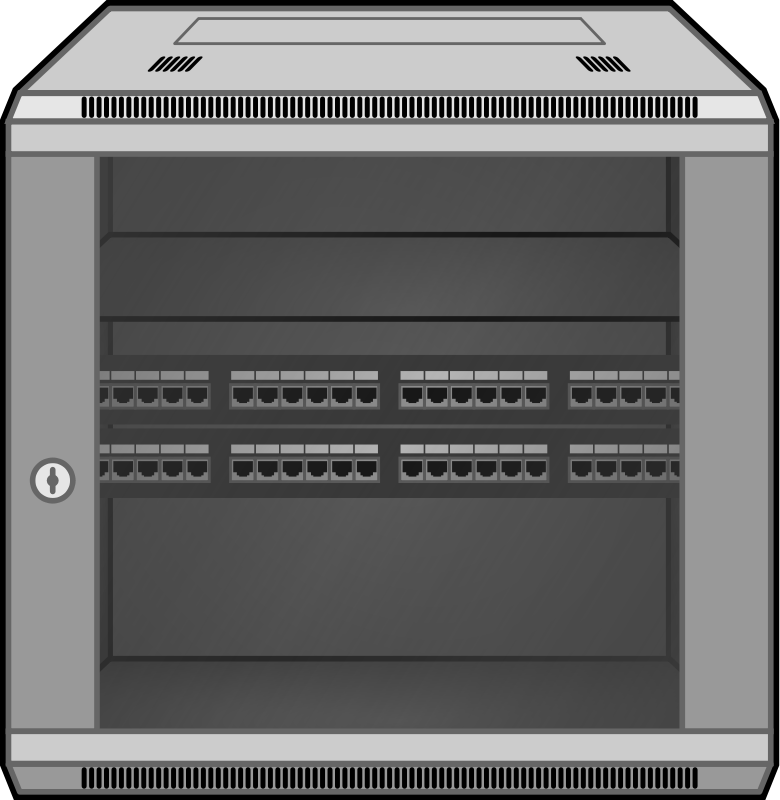
\includegraphics[width=2.5cm]{rack-system.png}};
        \node[above=0cm of rack-system, font=\footnotesize] {Модель};
        \node[cloud, draw, aspect=1.5, text width=3.2cm] at (rack-system) (cloud) {};
        
        \node[right=2cm of rack-system, yshift=-1cm] (laptop) {
\includegraphics[width=2.2cm]{laptop.png}};
        \node[color=white, anchor=base, font=\footnotesize, yshift=0.2cm] at (laptop) {\textbf{Симулятор}};
        
        \path[] (cloud) -- (laptop) node[draw, pos=0.6, sloped, single arrow, text width=0.4cm] {};
    \end{tikzpicture}
    \caption[Основная идея симуляции]{Основная идея симуляции. Модель некоторой вычислительной системы в виде программы исполняется на компьютере другой конфигурации и/или архитектуры}
    \label{fig:idea}
\end{figure}
\setcounter{chapter}{0} % restore the chapter counters
\setcounter{figure}{0}

Существует несколько различных трактовок терминов \textit{симуляция} и \textit{эмуляция}. Наиболее общеупотребительное понимание различия между ними таково: симуляция --- некий процесс, имитирующий внешние проявления системы, внутреннее его устройство при этом не повторяет детально оригинал; эмуляция же, кроме внешних эффектов, представляет внутреннюю структуру, максимально приближенную к оригинальной системе. Размышляя над этими определениями, можно заметить, что смысловая грань между ними очень тонка и в основном зависит от того, насколько глубоко мы готовы <<заглянуть>> в модель и в объект моделирования при исследовании; при этом эмуляция может легко оказаться симуляцией. По этой причине далее всюду в тексте понятия \textit{симулятор}, \textit{эмулятор}, \textit{модель} будут использоваться взаимозаменяемо, и их значение будет больше зависеть от контекста обсуждения, чем от строгих определений.

Существующие модели ЭВМ характеризуются и различаются множеством параметров, таких как фокусировка на различных аспектах работы изучаемой системы, точность соответствия поведения реальной и моделируемой системы, скорость работы, внутренний дизайн и внешние интерфейсы к нему, задействование различных оптимизационных техник и др. Изучение этих вопросов и составляет цель данной работы.

Для максимально эффективного усвоения материала книги читателю рекомендуется иметь начальные знания по архитектуре ЭВМ; рекомендуется обратиться к великолепной книге~\cite{patterson2012rus}. Желательно понимание читателем общих принципов работы операционных систем, а также знакомство как  минимум с одним языком программирования.

Нельзя не упомянуть книгу о виртуальных машинах, которая вдохновила авторов на написание этой работы~\cite{DBLP:books/daglib/0013597}. Знакомство с ней также настоятельно рекомендуется всем читателям, желающим глубже разобраться в вопросе виртуализации.

Необходимо понимать, что методика моделирования применима не только к изучению вычислительных или цифровых, но и практически к любых технических, социальных или каких-либо иных систем. Читателю, желающему расширить своё понимание метода, рекомендуется книга~\cite{system-modeling}.

В главе~\ref{chapter01} дано описание областей применения симуляторов, введены ключевые понятия и приведены примеры использования технологии симуляции в прошлом и в настоящее время.

%В главе~\ref{chapter02} описаны существующие в настоящее время программные решения, используемые в исследованиях, разработке и коммерческой эксплуатации.

В главе~\ref{chapter03} приводится пример построения простого симулятора процессора, основанного на интерпретации инструкций.

В главе~\ref{chapter04} представлены дальнейшие пути увеличения скорости моделей процессоров, такие как двоичная трансляция и аппаратная виртуализация.

В главе~\ref{chapter05} рассматривается исследование вычислительных систем с помощью трасс исполнения --- записи истории внешних событий.

%Глава~\ref{chapter06} знакомит с альтернативными подходами изучения ЭВМ с помощью различных методик: теории сетей центров обслуживания; сбора и проигрывания трасс событий; вероятностного моделирования.

Глава~\ref{chapter07} описывает подходы к симуляции системы с множеством устройств, включая многопроцессорные системы.

В главе~\ref{chapter08} рассматриваются подходы к параллельной симуляции; показывается, что эффективная и корректная реализация таких систем возможна, но в общем случае довольно сложна.

В главе~\ref{chapter09} описан подход к потактовой симуляции, обусловленный иным характером обработки событий в системе и потому отличный от ранее рассмотренных.

В главе~\ref{chapter10} показываются примеры организации хранилищ внутреннего состояния устройств, а также возможные для них оптимизации.

В главе~\ref{chapter11} кратко рассматриваются назначение и устройство сверхоперативной памяти (кэш-память), а также подходы к её моделированию.

В главе~\ref{chapter12} определяются существующие языки, используемые для написания моделей устройств, а также показывается их связь с языками, задействованными на поздних фазах, при проектировании устройств.

Глава~\ref{chapter13} знакомит с особенностями обеспечения взаимодействия симуляции с внешним физическим миром.

В главе~\ref{chapter14} даётся теоретический критерий возможности эффективной виртуализации вычислительных систем; затем проверяется соответствие ряда современных архитектур процессоров этому условию.


\newpage

\section*{Обозначения}

Всюду в тексте данной книги применяются следующие шрифтовые выделения и обозначения.

\begin{itemize*}
    \item Обычный текст используется для основного материала.
    \item \texttt{Моноширинный текст} вводится для исходных текстов программ на различных (псевдо)языках программирования, выделения ключевых слов, имён регистров устройств, листингов машинного кода.
    \item \textit{Наклонный текст} служит для выделения новых понятий.
    \item Числа в шестнадцатеричной системе счисления имеют префикс \textbf{0x} (например, 0x12345abcd), в двоичной системе счисления --- суффикс \textbf{b} (например, 10010011b).
\end{itemize*}

При введении терминов, заимствованных из английского языка и не имеющих известных авторам общепринятых переводов на русский, в скобках после них будут указываться оригинальные иностранные выражения.

\begin{digression}
    Параграфы, оформленные таким образом, являются необязательными для понимания курса и введены для того, чтобы показать порой неочевидные связи между приёмами моделирования и различными научными идеями и теориями.
\end{digression}

\iftoggle{webpaper}{
    \printbibliography[title={Литература}]
}{}

